\documentclass[11pt,a4paper]{jsarticle}
\usepackage[dvipdfmx]{graphicx}
\usepackage[utf8]{inputenc}
\title{横スクロールアクション仕様書}
\begin{document}
\maketitle

\section{要件定義}
\noindent
ゲームタイトル「高難度横スクロールアクション(仮)」

\subsection{開発概要}
インタプリタ言語Pythonを用いて横スクロール系アクションゲームを開発する。\\
横スクロール系アクションゲームとはプレイヤーがキャラクターを操作して、
道中の障害を回避しながらゴールへとたどり着くゲームである。本ゲームは挑戦回数を無制限とし、
プレイヤーがいかにして死亡回数が少ない状態でゴールにたどり着くかを競うゲームである。

プレイヤーは予め設定されたゴールを目指し、キーボードを使ってキャラクターを操作する。
キャラクターは移動、ジャンプ、攻撃、ダッシュ(素早く移動)ができる。
キャラクターはステージ上のアイテム拾うと使用することができる。

本ゲームは難易度が高く、ゴールするだけでも達成感がある構想である。
死亡回数がカウントされるため、死亡回数をどれだけ少なくできるか他プレイヤーと競い合える。
プレイヤーはキーボード操作で直感的にゲームを楽しむことができる。
ゲームの経験が浅い人でも楽しめるよう、キャラクターの操作やゲーム上のオブジェクトは最低限のシンプルな構成になっている。

\section{基本設計}
\subsection{ムービングオブジェクトや制限の概要}
\begin{itemize}
\item 落とし穴。キャラクターが落下した場合死亡する.。
\item エネミー。キャラクターが触れた場合死亡する。キャラクターの攻撃がエネミーに当たった場合エネミーは消滅する。
\item アイテム。ステージ上に存在し、キャラクターが使用すると死亡回数が1減る
\item ゴール地点の旗(?)。キャラクターの位置が旗と重なるとゲームクリアの判定が返される。
\item 制限時間。もし時間が0になってしまった場合死亡する。
\item 死亡と死亡回数。死亡した場合一度進行状況がリセットされ、ステージの最初から再開する。死亡する度に死亡回数が1増加する。
\end{itemize}

\subsection{キャラクターの挙動}
\begin{itemize}
\item 左右矢印キーをその方向にキャラクターが移動する。
\item スペースキーを押すとキャラクターがジャンプする。
\item 移動やジャンプには重力と慣性がはたらく。
\item シフトキーと左右矢印キーを同時に押すとキャラクターがその方向に素早く移動する。
\item Zキーを押すとキャラクターの前方にエネミーを攻撃する玉を発射する。
\item アイテムに触れるとそれを使用する。
\end{itemize}

\subsection{ゲーム画面の推移}
まず、プログラムを実行したとき初めに出てくるホーム画面を実装する。
ホーム画面ではゲームを開始する「GAME START」と、プログラム自体を終了する「EXIT」が選択できる。
ホーム画面で「START」を選択すると、ゲームのプログラムが実行される。
プレイヤーはキャラクターを操作して、障害物を避けながらゴールを目指す。
プレイヤーがゴールへたどり着くと、死亡回数やクリアタイムなどの結果がリザルト画面に表示される。
Enterキーを入力するとGAME START画面にもどる。

次ページに、画面推移のイメージ図を掲載した。

\begin{figure}[htbp]
	\centering
	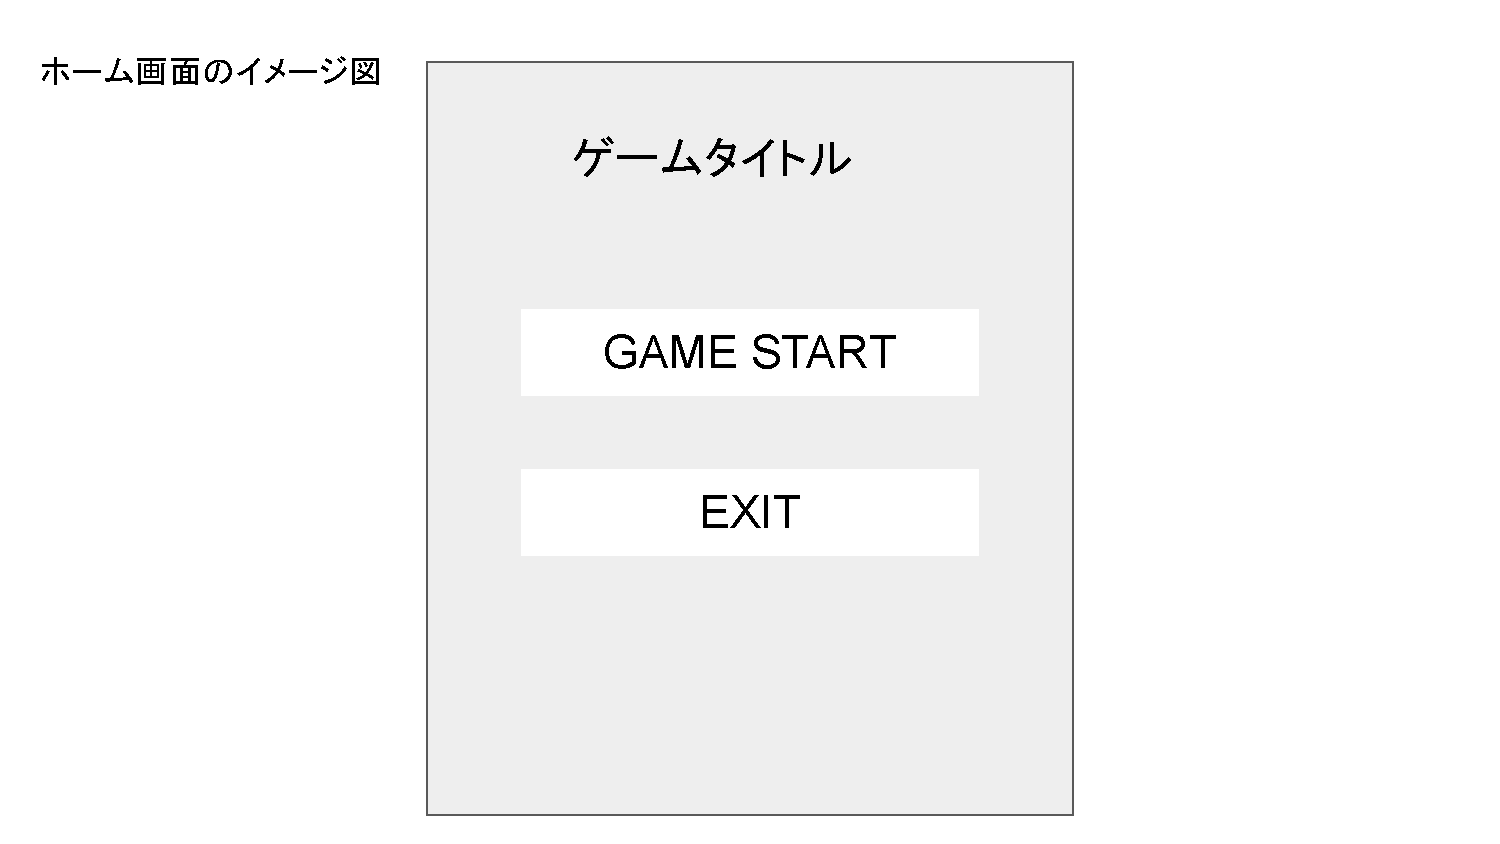
\includegraphics[width=110mm]{1.pdf}
	\caption{タイトル画面のイメージ}
	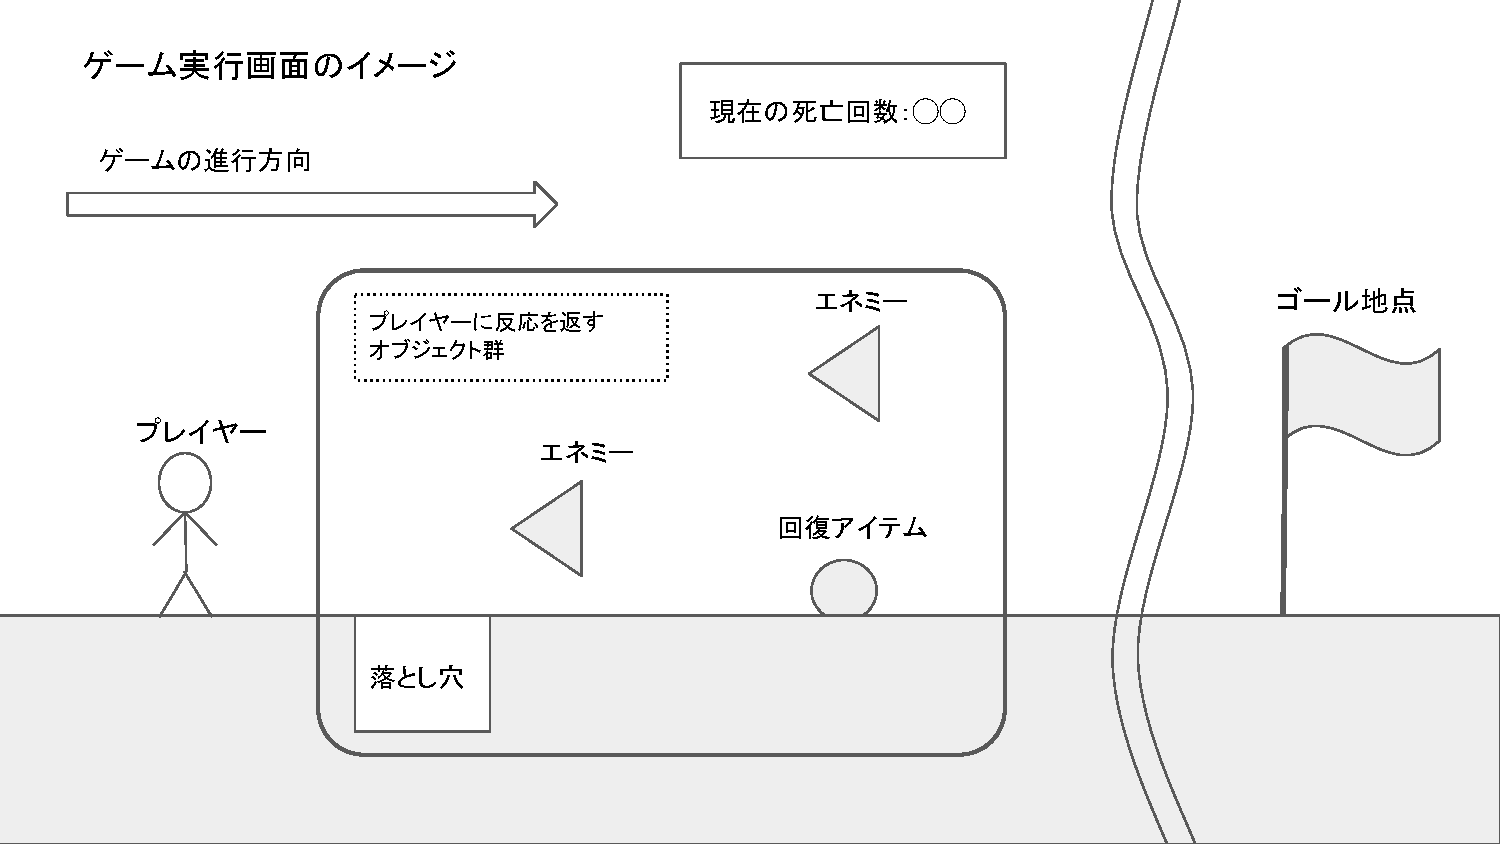
\includegraphics[width=110mm]{2.pdf}
	\caption{ゲーム画面のイメージ}
	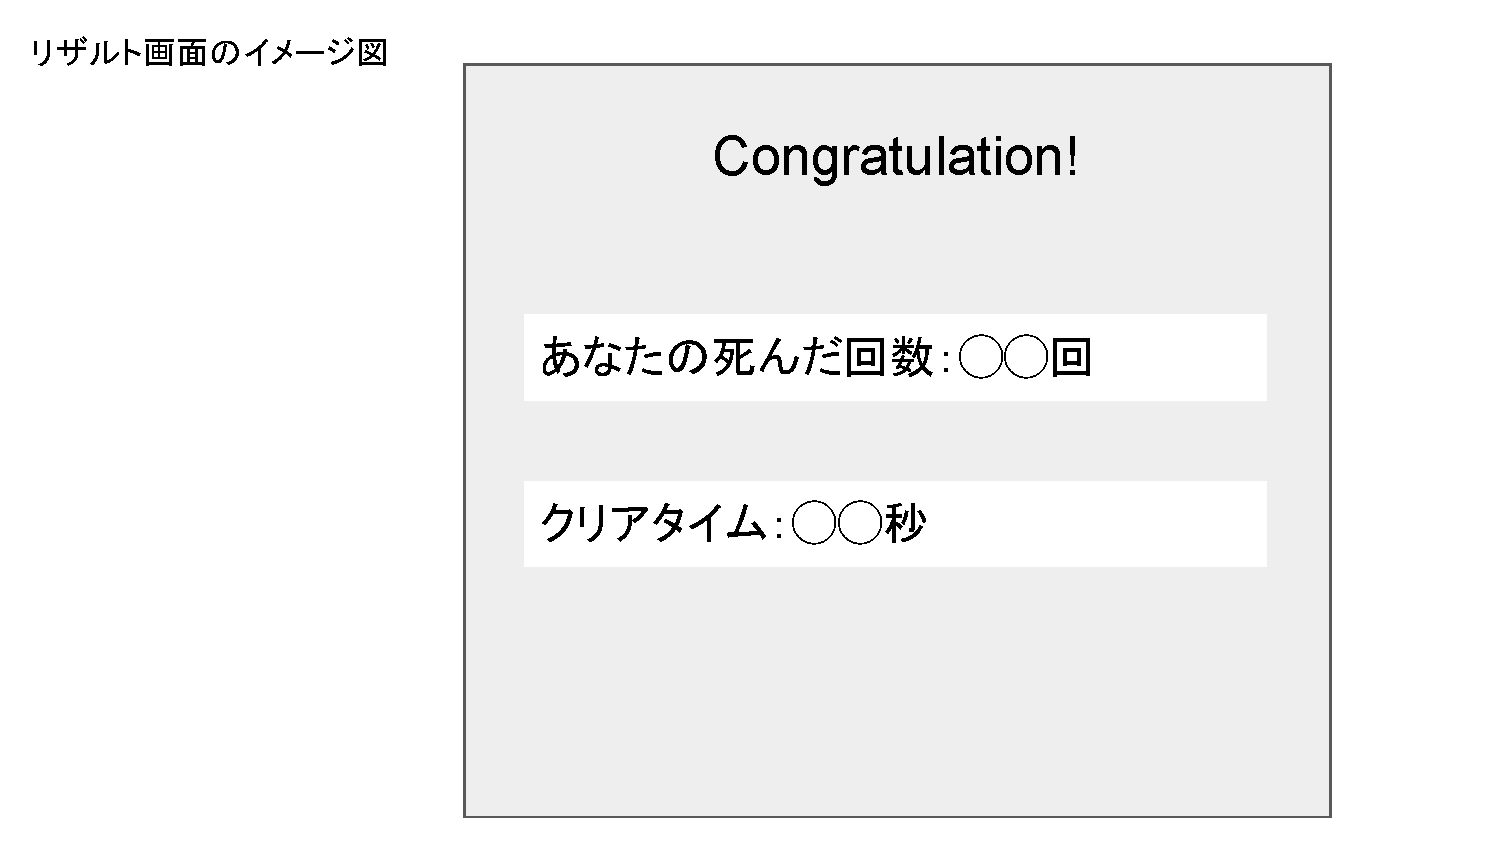
\includegraphics[width=110mm]{3.pdf}
	\caption{クリア画面のイメージ}
\end{figure}
\clearpage
\section{詳細設計}

\begin{figure}[htbp]
	\centering
	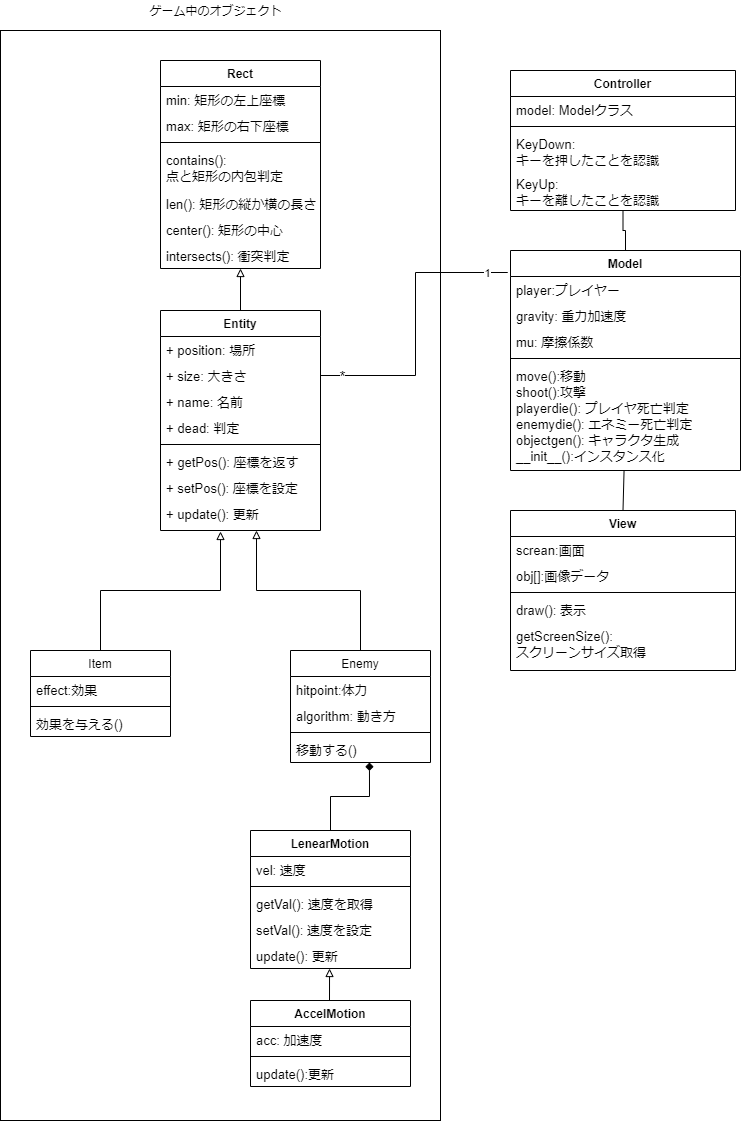
\includegraphics[width=110mm]{class.png}
	\caption{クラス図}
\end{figure}

\end{document}